\documentclass[1p]{elsarticle}

\usepackage{amsmath}
\usepackage{amssymb}
\usepackage{graphicx}
\usepackage{subfigure}
\usepackage[colorlinks,unicode,linkcolor=black]{hyperref}
\usepackage{listings}
\lstset{
    language=C++,
    basicstyle=\small,
    columns=flexible,
    showstringspaces=false,
    numbers=left,
    numberstyle=\tiny,
    frame=single
    }
\newcommand{\code}[1]{\lstinline|#1|}
\newcommand{\figref}[1]{Fig.~\ref{#1}}

%
% mathematical commands
%
\newcommand {\re} {\text{Re}}
\newcommand {\im} {\text{Im}}
\newcommand {\de} {\mbox{d}}
\newcommand {\ii} {\text{i}}
\newcommand {\ee} {\text{e}}
\newcommand {\mathbi}[1] {\textbf{\em #1}}
\newcommand {\sign} {\text{sign}}
\newcommand {\bra}[1] {\langle #1 \mid}
\newcommand {\ket}[1] {\mid #1 \rangle}
\newcommand {\braket}[2] {\langle #1 \mid #2 \rangle}
\newcommand {\mean}[1] {\langle #1 \rangle}
\newcommand {\sech} {\text{sech}}
\newcommand {\conj} {\ast}

\newcommand {\rem}[1]{}


\journal{Journal of Parallel and Distributed Computing}

\begin{document}

\begin{frontmatter}

\title{Programming OpenCL and CUDA:\\a Case Study Using Modern C++ Libraries}

\author{Karsten Ahnert}
\ead{karsten.ahnert@gmx.de}
\address{
Institut f\"ur Physik und Astronomie, Universit\"at Potsdam,\\
Karl-Liebknecht-Strasse 24/25, 14476 Potsdam-Golm, Germany
}

\author{Denis Demidov}
\ead{ddemidov@ksu.ru}
\address{
Kazan Branch of Joint Supercomputer Center,
Russian Academy of Sciences,\\
Lobachevsky st. 2/31, 420008 Kazan, Russia
}

\author{Karl Rupp}
\ead{rupp@iue.tuwien.ac.at}
\address{
Institute for Microelectronics, TU Wien,\\
Gusshausstrasse 27-29/E360, A-1040 Wien, Austria
}

\begin{abstract}
    We present comparison of several modern C++ libraries intended for
    OpenCL and CUDA programming. The comparison is based on odeint~---
    a framework for solution of ordinary differential
    equations. Odeint is designed in a very flexible way such that the
    algorithms are completely independent from the underlying
    containers and even from the basic algebraic computations. This
    allows to effectively use such libraries as VexCL, ViennaCL or
    Thrust to solve ODEs with either OpenCL or CUDA technologies. We
    found that OpenCL and CUDA work equally well for problems of large
    sizes. OpenCL has higher overhead for smaller problems, but allows
    on the fly generation of more effectice kernels.
\end{abstract}

\begin{keyword}
    GPGPU \sep OpenCL \sep CUDA \sep Modern C++ libraries
\end{keyword}

\end{frontmatter}





%
% INTRODUCTION
%
\section{Introduction}

Recently, GPGPU based computing has acquired considerable momentum in
scientific community. This is confirmed both by increasing numbers of
GPGPU-related publications and GPU based supercomputers in
the Top 500\footnote{\href{http://top500.org/}{http://top500.org/}} list. Major
programming frameworks are NVIDIA CUDA and OpenCL.  The former is proprietary
parallel computing architecture developed by Nvidia for general purpose
computing on Nvidia graphics cards, and the latter is open, royalty-free
standard for cross-platform, parallel programming of modern processors backed
by Khronos group. The frameworks have their distinctive pros and cons. CUDA has
more mature programming environment with larger set of scientific libraries;
but it is only supported on NVIDIA hardware. OpenCL is an open standard
supported on wide range of hardware but its native API requires much larger
amount of boilerplate code from a developer.

Both technologies are able to provide scientists with vast computational
resources of modern GPU cards. But the power comes with a price: GPGPU
programming has a steep learning curve. Programmer needs to familiarize
himself with (slightly) new programming language and, more importantly, with
new programming paradigm. However, the entry price may be lowered with help of
specialized libraries. CUDA Toolkit includes several such libraries (BLAS
implementation, Fast Fourier Transform, Thrust and others). OpenCL lacks
standard libraries, but there there are number of third party projects aimed at
both CUDA and OpenCL ease of development.

This paper presents comparison of several modern C++ libraries aimed at ease of
GPGPU development. We look at both convenience and performance of the libraries
under consideration in the context of solving ordinary differential equations.
The comparison is based on odeint~--- modern C++ library for solution of ODEs.
Odeint is designed in a very flexible way such that the algorithms are
completely independent from the underlying containers and even from the basic
algebraic computations. This allows to effectively use libraries implementing
basic linear algebra operations with either OpenCL or CUDA technologies for
solution of ODEs.



\begin{description}
    \item[Odeint] is a modern C++
        library\footnote{\href{http://odeint.com}{http://odeint.com}} for
	numerically solving Ordinary Differential Equations \cite{OdeintRef1,
	OdeintRef2}. It is developed in a generic way using Template
	Metaprogramming which leads to extraordinary high flexibility at top
	performance. The numerical algorithms are implemented independently of
	the underlying arithmetics.  This results in an incredible
	applicability of the library, especially in non-standard environments.
	For example, odeint supports matrix types, arbitrary precision
	arithmetics and can be easily adopted to use either CUDA or OpenCL
	frameworks.  Odeint is used in this work as a framework for comparison
	of other libraries.
    \item[Thrust] is a parallel algorithms
        library\footnote{\href{http://thrust.github.com}{http://thrust.github.com}}
	which resembles the C++ Standard Template Library \cite{ThrustRef}.
	Thrust's high-level interface greatly enhances developer productivity
	while enabling performance portability between GPUs and multicore CPUs.
	Thrust is distributed with NVIDIA CUDA Toolkit since version 4.1.
    \item[VexCL] is vector expression template
        library\footnote{\href{https://github.com/ddemidov/vexcl}{https://github.com/ddemidov/vexcl}}
	for OpenCL \cite{VexCLRef}. It has been created for ease of OpenCL
	development with C++.  VexCL strives to reduce amount of boilerplate
	code needed to develop OpenCL applications. The library provides
	convenient and intuitive notation for vector arithmetic, reduction, and
	sparse matrix-vector multiplication.  Multi-device and even
	multi-platform computations are supported. 
    \item[ViennaCL] (The Vienna Computing Library) is a scientific computing
        library\footnote{\href{http://viennacl.sourceforge.net}{http://viennacl.sourceforge.net}}
	written in C++ and based on OpenCL \cite{ViennaCLRef}. It allows
	simple, high-level access to the vast computing resources available on
	parallel architectures such as GPUs and is primarily focused on common
	linear algebra operations (BLAS levels 1, 2 and 3) and the solution of
	large systems of equations by means of iterative methods with optional
	preconditioner.
\end{description}

%Odeint supports Thrust and VexCL natively, but for ViennaCL we needed to
%provide adaptation code. Since ViennaCL already supports expression templates
%it can directly be used with the \code{vector_space_algebra} of odeint. There
%is no need to introduce an additional algebra or new operations. So in order to
%use \code{viennacl::vector} with odeint we only only needed to adapt the
%resizing operation. Resizing in odeint is necessary since many solvers need
%temporary state types. These state types need to be constructed and initialized
%which is done by the resizing mechanism of odeint.
%
%The resizing mechanism of odeint consist of three class templates. These
%classes are \code{is_resizeable<>} which is simply a meta function telling
%odeint if the type is really resizable. The second class is
%\code{same_size_impl<>} which has a static method \code{same_size} taking two
%\code{state_type} instances as arguments and returning if both instances have
%the same size. The third class is \code{resize_impl<>} which performs the
%actual resizing. These classes have a default implementation and can be
%specialized for any type.  For ViennaCL the specialization is very simple and
%is presented on \figref{fig:adapt:viennacl}.
%
%We were only able to test damped harmonic oscillator example with ViennaCL,
%since the library lacks such vector operations as elementwise multiplication or
%function application necessary for the other examples.  Nevertheless we
%consider comparison with ViennaCL interesting enough to include in this paper.
%Indeed, ViennaCL and VexCL employ somewhat different approaches to OpenCL
%kernel generation. ViennaCL has limited number of kernels, which coincide
%functionally with BLAS level 1 routines. These kernels are compiled in batch at
%the program start to allow for faster initialization. However, due to this
%design decision each vector expression may result in launch of more than one
%kernel.  On the other hand, VexCL generates and compiles single kernel for each
%vector expression it encounters.  This leads to higher initialization overhead,
%but should prove more effective in the long runs. It should be noted that main
%aim of ViennaCL is provision of iterative solvers for large sparse systems of
%equations. In this context complex vector expressions are rare and we think
%that authors of ViennaCL made correct design decision.  However, we think it is
%interesting to compare approaches of VexCL and ViennaCL.









%
% ADAPTING ODEINT
%
\section{Adapting odeint}

\begin{figure}
\begin{lstlisting}
typedef std::array<double, 3> state_type;
state_type x1, x2;
// Initialize x1 and x2.

double dt = 0.1;
odeint::range_algebra algebra;
// The following line computes x1 = dt * x2 for all elements of x1 and x2:
algebra.for_each2(x1, x2, default_operations::scale_sum1(dt));
\end{lstlisting}
\caption{An example of range algebra in odeint.}
\label{fig:odeintops}
\end{figure}

Odeint provides a mechanism which lets the user change the way how the
elementary numerical computations are performed. This mechanism consists of a
combination of state type, algebra and operations. State type represents the
state of the ODE being solved and is usually a vector type like
\code{std::vector<>} or \code{std::array<>}. The algebra is responsible for
iterating through all elements of the state whereas the operations are
responsible for the elementary operations. \figref{fig:odeintops} provides an
example of using range algebra. Here \code{for_each2} is used, which means that
two state types are iterated. The operation is a \code{scale_sum1} which simply
calculates \code{x1[i] = dt * x2[i]}. Odeint provides a set of predefined
algebras, which includes:
\begin{itemize}
    \item \code{range_algebra}: default algebra which works on Boost.Ranges
    \item \code{array_algebra}: specialized algebra for boost::array
    \item \code{fusion_algebra}: algebra for compile-time sequences like
        \code{boost::fusion::vector}, \code{std::tuple}, etc.
    \item \code{vector_space_algebra}: algebra for vector space types which
        provide overloaded arithmetic operators for elementwise operations.
\end{itemize}

Many libraries for vector and matrix types provide expression templates for the
elementary operations. Such libraries do not need an own algebra but can be
used with the \code{vector_space_algebra} and the \code{default_operations}
which simply calls the operations directly on the matrix or vector type. In
this case only odeint resizing mechanism has to be adapted.

In the following subsections we describe odeint adaptation for GPGPU libraries
under consideration. We should mention that odeint now supports all of the
mentioned libraries natively. However, providing adaptation examples serves our
goal of comparing ease of use of the libraries.

\subsection{Thrust}
\subsection{VexCL}
\subsection{ViennaCL}














\section{Numerical experiments}

typical use cases of solving ODEs on GPU, parameter studies, large systems, discretization of PDEs...





%
% DAMPED OSCILLATOR
%
\subsection{Damped Harmonic Oscillator Ensemble}

dependence on an external parameter (the time)
include $x^3$?

The first example is a set of damped driven oscillators 

\begin{equation} \label{eq:dampedsystem}
    \frac{\de x}{\de t} = \omega y + \varepsilon x, \quad 
    \frac{\de y}{\de t} = -\omega x + \varepsilon y.
\end{equation}

with $\varepsilon = \varepsilon_0 + \varepsilon_a \cos \left( \omega_d
t \right)$. $\omega$ is the natural frequency of the oscialltor and $\varepsilon$ is the time dependent daming constant. 
Note, that this form is not the classical form of a damped oscillator, but can be derived easily from $\ii \dot{\Psi} = \omega \Psi + \ii \varepsilon \Psi$ with $\Psi = x + \ii y$.


\figref{code:thrust:damped} shows Thrust version of the system functor for the
damped harmonic oscillator ensemble experiment. The functor holds model
parameters and provides \code{operator()} with signature required by odeint
library. The state type is represented by \code{device_vector<double>}.  First
part of the vector holds $x$-components of state, and second part holds
$y$-components. In the \code{operator()} components of state and state
derivative are packed into a zip iterator and passed to \code{for_each}
function together with provided device functor. In the functor individual
components are unpacked again and the operations required are applied to
derivative part. This technique allows to compute system function in single
efficient pass resulting in single CUDA kernel launch.

\begin{figure}[p]
\begin{lstlisting}
typedef thrust::device_vector<double> state_type;

struct oscillator {
    size_t N;
    double omega, amp, offset, omega_d;

    oscillator(size_t N, double omega, double amp, double offset, double omega_d)
        : N(N), omega(omega), amp(amp), offset(offset), omega_d(omega_d) { }

    struct oscillator_functor {
        double eps, omega;

        oscillator_functor(double omega, double eps)
            : omega(omega), eps(eps) {}

        template< class T >
        __host__ __device__ void operator()(T t) const {
            double x = thrust::get< 0 >( t );
            double y = thrust::get< 1 >( t );
            thrust::get<2>(t) = eps * x + omega * y;
            thrust::get<3>(t) = eps * y - omega * x;
        }
    };

    void operator()(const state_type &x, state_type &dxdt, double t) const {
        double eps = offset + amp * cos(omega_d * t);
        thrust::for_each(
            thrust::make_zip_iterator(
                thrust::make_tuple(
                    boost::begin(x),
                    boost::begin(x) + N,
                    boost::begin(dxdt),
                    boost::begin(dxdt) + N ) ),
            thrust::make_zip_iterator(
                thrust::make_tuple(
                    boost::begin(x) + N,
                    boost::begin(x) + 2 * N,
                    boost::begin(dxdt) + N,
                    boost::begin(dxdt) + 2 * N ) ),
            oscillator_functor(omega, eps) );
    }
};
\end{lstlisting}
\caption{System functor for Thrust version of damped harmonic oscillator
ensemble example.}
\label{code:thrust:damped}
\end{figure}

\figref{code:vexcl:damped} shows system functor for VexCL version of the damped
harmonic oscillator example. The functor looks much simpler than Thrust variant
because VexCL supports rich set of vector expression templates. The
state type is represented by \code{multivector<double,2>} which holds two
instances of \code{vex::vector<double>} and transparently dispatches all
operations to its underlying components. It would be in principle possible to
write the \code{operator()} body as
\begin{lstlisting}[frame=leftline]
double eps = offset + amp * cos(omega_d * t);
dxdt(0) = eps * x(0) + omega * x(1);
dxdt(1) = eps * x(1) - omega * x(0);
\end{lstlisting}
This would basically coincide with the problem statement
\eqref{eq:dampedsystem}. The drawback of this variant is that it would result
in two kernel launches (one per each vector assignment) and lead to suboptimal
performance. We also can not use simple multivector arithmetic operations here
because components in the right hand sides of the assignments are interchanged.
Fortunately, VexCL supports multi-operation notation. Assignment of a tuple of
expressions to a multivector leads to generation and launch of single efficient
OpenCL kernel. This notation is only marginally more cumbersome than the above
variant.

\begin{figure}[p]
\begin{lstlisting}
typedef vex::vector<double> vector_type;
typedef vex::multivector<double, 2> state_type;

struct oscillator {
    double omega, amp, offset, omega_d;

    oscillator(double omega, double amp, double offset, double omega_d)
        : omega(omega), amp(amp), offset(offset), omega_d(omega_d) { }

    void operator()(const state_type &x, state_type &dxdt, double t) const {
        double eps = offset + amp * cos(omega_d * t);

        dxdt = std::make_tuple(
                eps * x(0) + omega * x(1),
                eps * x(1) - omega * x(0) );
    }
};
\end{lstlisting}
\caption{System functor for VexCL version of damped harmonic oscillator
ensemble example.}
\label{code:vexcl:damped}
\end{figure}

\begin{figure}[p]
\begin{lstlisting}
typedef vex::vector<double> state_type;

extern const char oscillator_body[] = "return sin(X[-1] - X[0]) + sin(X[0] - X[1]);";

struct phase_oscillators {
    const state_type &omega;
    vex::StencilOperator< double, 3, 1, oscillator_body > S;

    phase_oscillators(const state_type &omega) : omega(omega), S(omega.queue_list()) { }

    void operator()(const state_type &x, state_type &dxdt, double t) const {
        dxdt = omega + S(x);
    }
};
\end{lstlisting}
\caption{System functor for VexCL version of coupled phase oscillators chain
example}
\label{code:vexcl:phase}
\end{figure}

The ViennCL version of the damped harmonic oscillator example is presented on
\figref{code:viennacl:damped}. \code{boost::fusion::vector} is used to pack
coordinate components of the state type (represented by
\code{viennacl::vector<double>} instances) into a single structure. We also had
to adapt odeint resizing mechanism to the resulting structure. Its
implementation is straightforward and omitted here for the sake of conciseness.

ViennaCL, as well as VexCL, supports expression templates for a limited set of
vector operations (closely corresponding to Level 1 BLAS routines). More
complex expressions may be built with help of ViennaCL kernel generator
interface, which supports single- or multiple-operations kernels. The required
notation is a bit more cumbersome than that of VexCL library. OpenCL kernels
here are generated from symbolic expressions involving explicit symbolic types.
This requires more of boilerplate code but the resulting expression tree
carries information of whether two terminals represent the same vector
instance. This in principle allows generation of more effective code.

\begin{figure}[p]
\begin{lstlisting}
typedef viennacl::vector<double> vector_type;
typedef fusion::vector<vector_type, vector_type> state_type;

struct oscillator {
    double omega, amp, offset, omega_d;

    viennacl::generator::symbolic_vector<0, double> sym_dx;
    viennacl::generator::symbolic_vector<1, double> sym_dy;
    viennacl::generator::symbolic_vector<2, double> sym_x;
    viennacl::generator::symbolic_vector<3, double> sym_y;
    viennacl::generator::cpu_symbolic_scalar<4, double> sym_eps;
    viennacl::generator::cpu_symbolic_scalar<5, double> sym_omega;
    viennacl::generator::custom_operation op;

    oscillator(double omega, double amp, double offset, double omega_d)
        : omega(omega), amp(amp), offset(offset), omega_d(omega_d),
          op(sym_dx = sym_eps * sym_x + sym_omega * sym_y,
             sym_dy = sym_eps * sym_y - sym_omega * sym_x,
             "oscillator")
    { }

    void operator()( const state_type &x, state_type &dxdt, double t ) {
        vector_type &X = const_cast<vector_type&>( fusion::at_c<0>(x) );
        vector_type &Y = const_cast<vector_type&>( fusion::at_c<1>(x) );

        vector_type &dX = fusion::at_c<0>(dxdt);
        vector_type &dY = fusion::at_c<1>(dxdt);

        double eps = offset + amp * cos(omega_d * t);

        viennacl::ocl::enqueue( op(dX, dY, X, Y, eps, omega) );
    }
};
\end{lstlisting}
\caption{System functor for ViennaCL version of damped harmonic oscillator
ensemble example.}
\label{code:viennacl:damped}
\end{figure}





%
% PHASE OSCILLATORS
%
\subsection{Chain of Coupled Phase Oscillators}

\rem{As a second example we choose a chain of coupled phase oscillators. A
phase oscillator describes the dynamics of an autonomous oscillator
\cite{Pikovsky-Rosenblum,Kuramoto,scholarpedia articles}. Its
evolutions is governed by the phase, a $2\pi$ periodic variable which
grows linearily in time $\de \phi / \de t = \omega$. $\omega$ is here
the phase velocity. Since the absence of any information about the
amplitude of the oscillator interesting behaviour can only be observed
if many of such oscillators are coupled. In fact such system can be
used to study such divergent phenomena like synchronization, wave and
pattern formation, phase chaos, or oscillation death \cite{}. It is a
prominent example of an emergent system where the coupled system shows
more complex behaviour than its constitutes.

The concrete example we analyze here is a chain of nearest-neighbor
coupled phase oscillators:
\begin{equation}
    \frac{\de \phi_i}{\de t} = \omega_i + \sin( \phi_{i+1} - \phi_i) + \sin( \phi_i
    - \phi_{i-1}).
\end{equation}
The index $i$ denotes here the $i$-th phase in the chain. Note, that
the phase velocity might be heterogenous.
}



As a second example we choose a chain of coupled phase oscillators. Phase
oscillators are a very simplified version of usual oscillator where the state
is described by a $2\pi$ periodic variable. If a single phase oscillator is
uncoupled its phase $\phi$ is described by a linear growth $d\phi/dt = \omega$
where $\omega$ is the phase velocity. Therefore, interesting behavior can only
be observed if two or more oscillators are coupled. In fact, a system of
coupled phase oscillators is a prominent example of an emergent system where
the coupled system shows a more complex behavior than its constitutes.

The concrete example we analyze here is:
\begin{equation} \label{eq:phasesystem}
    \frac{d\phi_i}{dt} = \omega_i + \sin( \phi_{i+1} - \phi_i) + \sin( \phi_i
    - \phi_{i-1}).
\end{equation}
Note that $\phi_i$ is a function of the time, the index $i$ denotes here the
$i$-th phase in the chain.

Thrust version for the coupled phase oscillator chain looks very similar to the
damped oscillator example. Again, we use zip iterator to pack required
components and process the resulting sequence with single sweep of
\code{for_each} algorithm. The only difference here is that we need values of
neighboring vector elements. In order to provide the values, we use Thrust's
permutation iterator, so that \code{operator()} of the system functor looks
like
\begin{lstlisting}[frame=leftline]
thrust::for_each(
    thrust::make_zip_iterator(
        thrust::make_tuple(
            x.begin(),
            thrust::make_permutation_iterator( x.begin(), prev.begin() ),
            thrust::make_permutation_iterator( x.begin(), next.begin() ),
            omega.begin(),
            dxdt.begin() ) ),
    thrust::make_zip_iterator(
        thrust::make_tuple(
            x.end(),
            thrust::make_permutation_iterator( x.begin(), prev.end() ),
            thrust::make_permutation_iterator( x.begin(), next.end() ),
            omega.end(),
            dxdt.end() ) ),
    sys_functor()
    );
\end{lstlisting}
\code{prev} and \code{next} are instances of
\code{thrust::device_vector<size_t>} holding indices to left and right vector
elements and initialized as
\begin{lstlisting}[frame=leftline]
thrust::counting_iterator<size_t> c(0);
thrust::copy(c, c + N - 1, prev.begin() + 1);
prev[0] = 0;     // prev = { 0, 0, 1, 2, 3, ..., N-1 }
thrust::copy(c + 1, c + N, next.begin());
next[N-1] = N-1; // next = { 1, 2, 3, ..., N-1, N-1 }
\end{lstlisting}

VexCL version of the example is presented on \figref{code:vexcl:phase}. Again,
it is the most concise variant since VexCL provide native support for the
user-defined stencils operations. The sum of sines in \eqref{eq:phasesystem} is
encoded in \code{StencilOperator} class template. Template parameters are
string for body of the generated OpenCL function encoding required operation;
width and center point of the stencil and its return type. Once the stencil
operator is defined, the functor's \code{operator()} is programmed with a
single of code.

\figref{code:viennacl:phase} presents ViennaCL version of the phase oscillator
chain example. Unfortunately, ViennaCL does not provide operations required for
the problem at hand, so we had to fallback to hand-coded OpenCL kernel.
ViennaCL provide convenient mechanism for compilation and launching of custom
kernels, so this was a pleasant experience in comparison with native OpenCL
API. This low-level variant expectedly turned out to be most effective as it
will be shown in Results section.

\begin{figure}[p]
\begin{lstlisting}
typedef viennacl::vector<double> state_type;

struct phase_oscillators {
    const state_type &omega;

    sys_func(const state_type &omega) : omega(omega) {
        static const char source[] =
            "#pragma OPENCL EXTENSION cl_khr_fp64: enable\n"
            "kernel void oscillator(\n"
            "        uint n,\n"
            "        global double *dx,\n"
            "        global const double *x,\n"
            "        global const double *omega\n"
            "        )\n"
            "{\n"
            "    for(uint i = get_global_id(0); i < n; i += get_global_size(0)) {\n"
            "        double X0 = x[i];\n"
            "        double Xl = i > 0 ? x[i - 1] : X0;\n"
            "        double Xr = i + 1 < n ? x[i + 1] : X0;\n"
            "        dx[i] = omega[i] + sin(Xl - X0) + sin(X0 - Xr);\n"
            "    }\n"
            "}\n";

        viennacl::ocl::current_context().add_program(
                source, "oscillator_program").add_kernel("oscillator");
    }

    void operator()(const state_type &x, state_type &dxdt, double t) const {
        viennacl::ocl::kernel &step = viennacl::ocl::current_context().get_program(
            "oscillator_program").get_kernel("oscillator");
        viennacl::ocl::enqueue(
            step(static_cast<cl_uint>(x.size()), dxdt, x, omega) );
    }
};
\end{lstlisting}
\caption{System functor for ViennaCL version of coupled phase oscillators chain
example}
\label{code:viennacl:phase}
\end{figure}










%
% DISORDERED LATTICES
%
\subsection{Disordered Ham Lattice}

\rem{
Another example for our performance and usage study is a strongly
nonlinear disordered Hamiltonian lattice. Its equations of motion are
governed by
\begin{equation}
\frac{\de q_{i,j}}{\de t} = p_{i,j} \quad \text{,} \quad \quad \frac{\de p_{i,j}}{\de t} = - \omega_{i,j}^2 q_i - \beta q_{i,j}^3 + \Delta_d q_{i,j} \,\,\text{.}
\label{eq:disordered_ham}
\end{equation}
Here, $\Delta_d q_{i,j}$ denotes the two-dimensional discret Laplacian
$\Delta_d
q_{i,j}=q_{i+1,j}+q_{i-1,j}+q_{i,j+1}+q_{i,j-1}-4q_{i,j}$. Such
systems are widely used in theoretical physics to study phenomena
like Anderson localization or thermalization.

An important property of \eqref{eq:disordered_ham} is its Hamiltonian
nature. It can be obtained from a Hamiltonian and the energy and phase
volume is conserved during its evolution. To account for this
properties a special class of solvers exists -- symplectic
solvers. Odeint implements three different variants of such solvers,
all are of the Runge-Kutta-Nystrom type.
}

\begin{equation} \label{eq:latticesystem}
    \frac{dp}{dt} = -\Delta Kq + Dq - \beta q^3.
\end{equation}

Natural choice for the implementation of \eqref{eq:latticesystem} is sparse
matrix vector product. Unfortunately, Thrust provides neither sparse matrix
type, nor sparse matrix~-- vector product operation.  We had to combine Thrust
with CUSPARSE library in order to implement this example. CUSPARSE library
contains a set of basic linear algebra subroutines used for handling sparse
matrices and is included in CUDA Toolkit distribution as well as Thrust
library.

All of the libraries we compared hold sparse matrix  representation in hybrid
ELL format. This is one of the most effective formats for sparse matrices on
GPUs~\cite{BellGarland2008}.

Linear operator $-\Delta Kx-Dx$ may be represented as a single sparse matrix.
The construction of the matrix is not very interesting in the context of this
paper, so we only provide code for the system functor's \code{operator()}.

Thrust version of the system functor looks like this:
\begin{lstlisting}[frame=leftline]
typedef thrust::device_vector<double> state_type;

void operator()(const state_type &q , state_type &dp) const {
    static double one = 1;
    thrust::transform(q.begin(), q.end(), dp.begin(),
	    scaled_pow3_functor(-beta) );
    cusparseDhybmv(handle, CUSPARSE_OPERATION_NON_TRANSPOSE, &one, descr, A,
	    thrust::raw_pointer_cast(&q[0]), &one,
	    thrust::raw_pointer_cast(&dp[0]) );
}
\end{lstlisting}
Here \code{handle}, \code{descr}, and \code{A} are CUSPARSE data structures
holding CUSPARSE context and sparse matrix data. In lines 5 and 6
\code{thrust::transform()} algorithm is used to compute scaled cube of input
vector \code{q}. Lines 7--9 call procedure for sparse matrix~-- vector product.
Function \code{thrust::raw_pointer_cast()} is used to convert thrust device
vector iterator to raw device pointer.

VexCL version looks very simple:
\begin{lstlisting}[frame=leftline]
typedef vex::vector<double> state_type;

extern const char pow3_body[] = "return prm1 * prm1 * prm1;";
vex::UserFunction<pow3_body, double(double)> pow3;

void ham_lattice::operator()(const state_type &q, state_type &dp) const {
    dp = (-beta) * pow3(q) + A * q;
}
\end{lstlisting}

User-defined OpenCL function \code{pow3} computes cube of its argument and is
presented here for the performance sake. \code{A} is \code{vex::SpMat<double>}
instance holding discretisation of linear operator $-\Delta Kx - Dx$.

ViennaCL neither supports elementwise vector product nor provides
overloaded math functions for its vector types. That's why we had to split its
\code{operator()} into two parts: the first part computes sparse matrix~--
vector product normally, while the second part uses hand-coded kernel to
subtract non-linear term $\beta q^3$ from the result:
\begin{lstlisting}[frame=leftline]
typedef viennacl::vector<double> state_type;

void ham_lattice::operator()(const state_type &q, state_type &dp) const {
    dp = viennacl::linalg::prod(A, q);

    viennacl::ocl::kernel &scaled_pow3 =
        viennacl::ocl::current_context().get_program(
                "pow3_program").get_kernel("scaled_pow3");

    viennacl::ocl::enqueue(
        scaled_pow3(static_cast<cl_uint>(q.size()), dp, q, beta) );
}
\end{lstlisting}











%
% LORENZ ATTRACTOR
%
\subsection{Lorenz Attractor Ensemble}

In the first example we will use the Lorenz system \cite{Lorenz}. The
Lorenz system is a system of three coupled ODEs which shows chaotic
behavior for a large range of parameters. It is one of the most used
toying ODE in the nonlinear dynamics community. The ODE of the Lorenz
system reads
\begin{align}
    \frac{\de x}{\de t} &= -\sigma \left( x - y \right), \\
    \frac{\de y}{\de t} &= R x - y - xz, \\
    \frac{\de z}{\de t} &= -bz + xy.
\end{align}

Interesting question around the Lorenz system usually arise with
dependence on one of its parameters. For example one might want to
study the dependence on the chaoticity on the parameter
$R$. Therefore, one would create a large set of Lorenz systems (each
with a different parameter $R$), pack them all into one system and
solve them simultaneously. (In a real study of chaoticity one would
usually calculate the Lyapunov exponents \cite{Benettin}, which
require to solve the system of Lorenz and their linear perturbations.)


In the first example we will use the Lorenz system and study its dependence on
one of the parameters. The Lorenz system is a system of three coupled ODEs
which shows chaotic behavior for a large range of parameters. The ODE reads
\begin{align}
    \frac{dx}{dt} &= -\sigma \left( x - y \right), \\
    \frac{dy}{dt} &= R x - y - xz, \\
    \frac{dz}{dt} &= -bz + xy.
\end{align}

We will study the dependence on the parameter $R$. Therefore, we create a large
set of these systems (each with a different parameter $R$), pack them all into
one system and solve them simultaneously on the GPU.

\section{Results}

We present results for the numerical experiments in this section. The complete
source code for the experiments and the full set of results may be found at
GitHub
repository\footnote{\href{https://github.com/ddemidov/vexcl_odeint_paper}{https://github.com/ddemidov/vexcl\_odeint\_paper}}.

All of the libraries we tested in this paper allow use of both CPU and GPU
compute paths. Thrust supports OpenMP based CPU path that is enabled by
compilation switch and OpenCL libraries natively support CPU as a compute
device.  The timings we provide here were obtained for Nvidia Tesla C2070 GPUs
and for Intel Core i7 930 CPU. For each of the experiments, 10 runs were made
and median time was selected as a representative value.

Figures \ref{fig:damped:perf} through \ref{fig:lorenz:perf} show performance
data for the four numerical experiments. Left plots shows absolute time with
against the size of the solved problem, while right plots show relative
performance with respect to Thrust GPU version.

In general all of the experiments show 10x to 20x acceleration when run on GPU
with respect to the CPU path. Both CUDA and OpenCL programs show considerable
overhead for the smaller sized problems. Due to this overhead we needed
problems of size $10^3-10^4$ to see any acceleration on GPU. The overhead for
OpenCL libraries is larger than that of CUDA programs. This is explained by the
fact that OpenCL program compiles its computational kernels at runtime.

VexCL library allows transparent use of several GPUs. \figref{fig:scaling}
shows scaling results for up to three Tesla GPUs. It is clear from the plots
that it does make sense to use several GPUs only for problems of size larger
than $10^5-10^6$. Additional advantage of multi-GPU programming model is that
memory resources are split between all of the GPUs so that larger problems may
be processed.

\begin{figure}[p]
    \begin{center}
        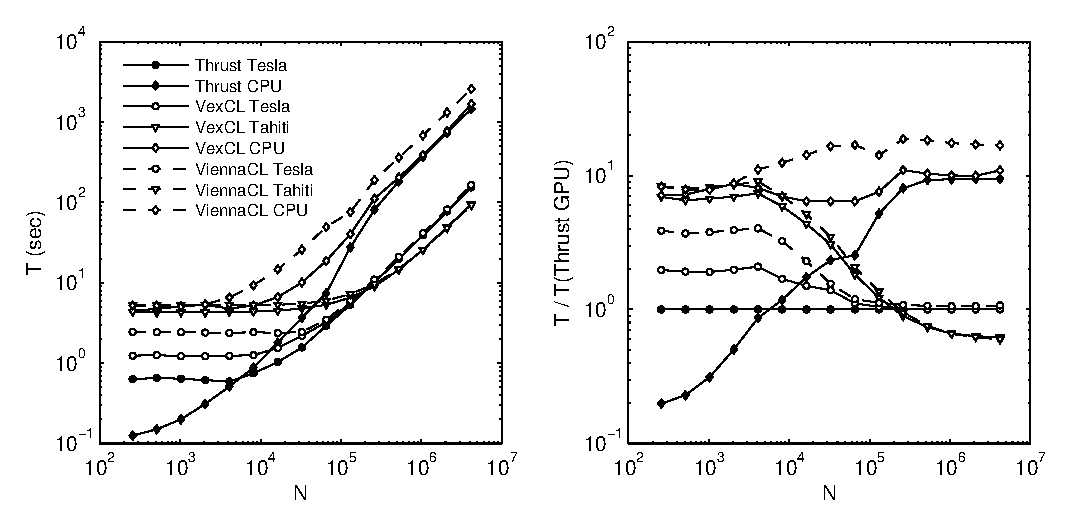
\includegraphics[width=\textwidth]{data/damped_oscillator/perfcmp}
    \end{center}
    \caption{Damped oscillator ensemble results}
    \label{fig:damped:perf}
\end{figure}

\begin{figure}[p]
    \begin{center}
        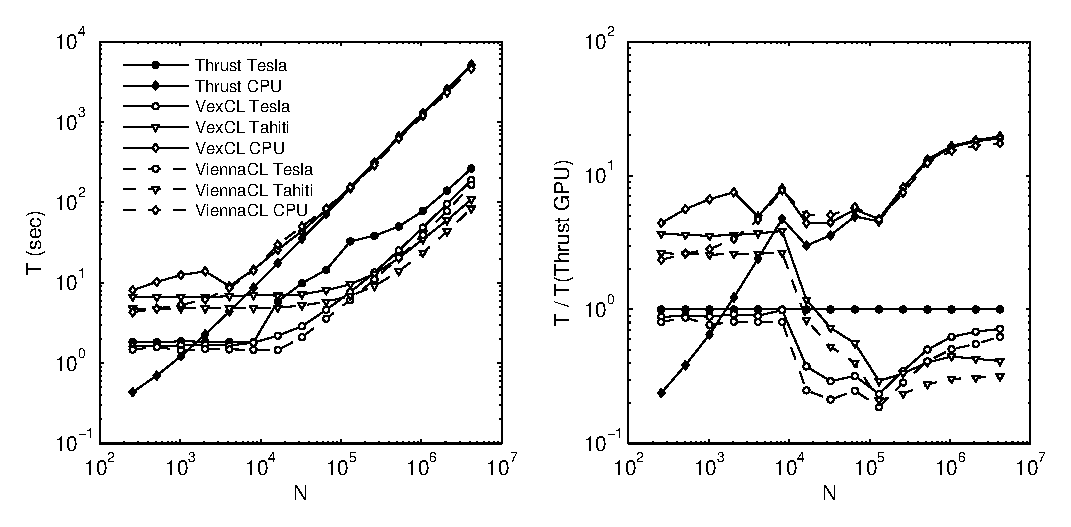
\includegraphics[width=\textwidth]{data/phase_oscillator_chain/perfcmp}
    \end{center}
    \caption{Coupled phase oscillator chain results}
    \label{fig:phase:perf}
\end{figure}

\begin{figure}[p]
    \begin{center}
        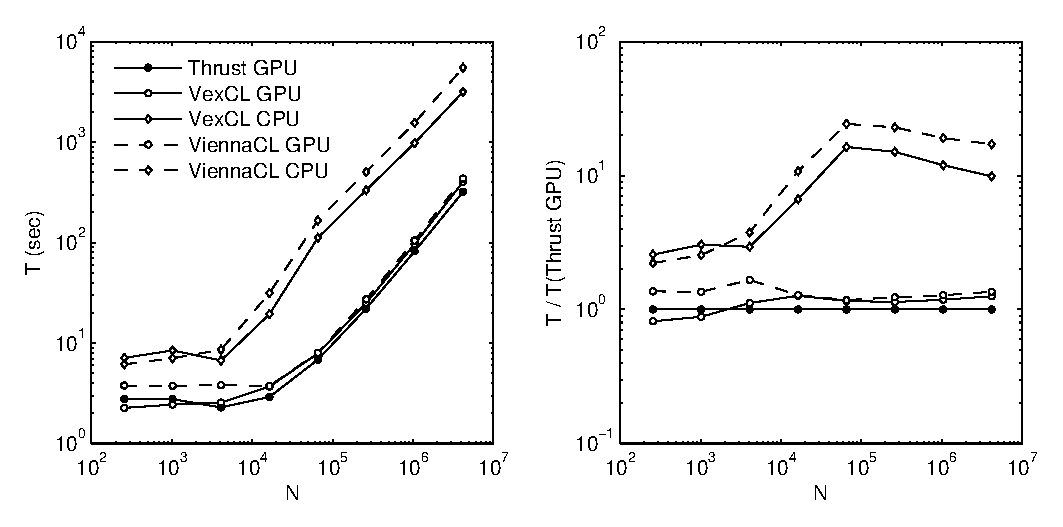
\includegraphics[width=\textwidth]{data/disordered_ham_lattice/perfcmp}
    \end{center}
    \caption{Disordered Ham lattice results}
    \label{fig:lattice:perf}
\end{figure}

\begin{figure}[p]
    \begin{center}
        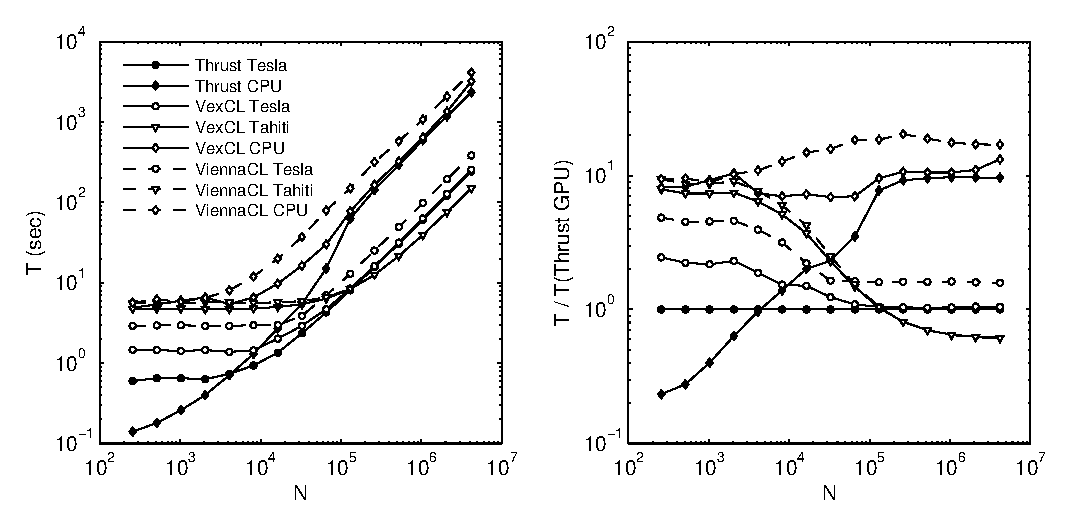
\includegraphics[width=\textwidth]{data/lorenz_ensemble/perfcmp}
    \end{center}
    \caption{Lorenz attractor ensemble results}
    \label{fig:lorenz:perf}
\end{figure}

\begin{figure}[p]
    \begin{center}
        \subfigure[
        Damped oscillator ensemble
        ]{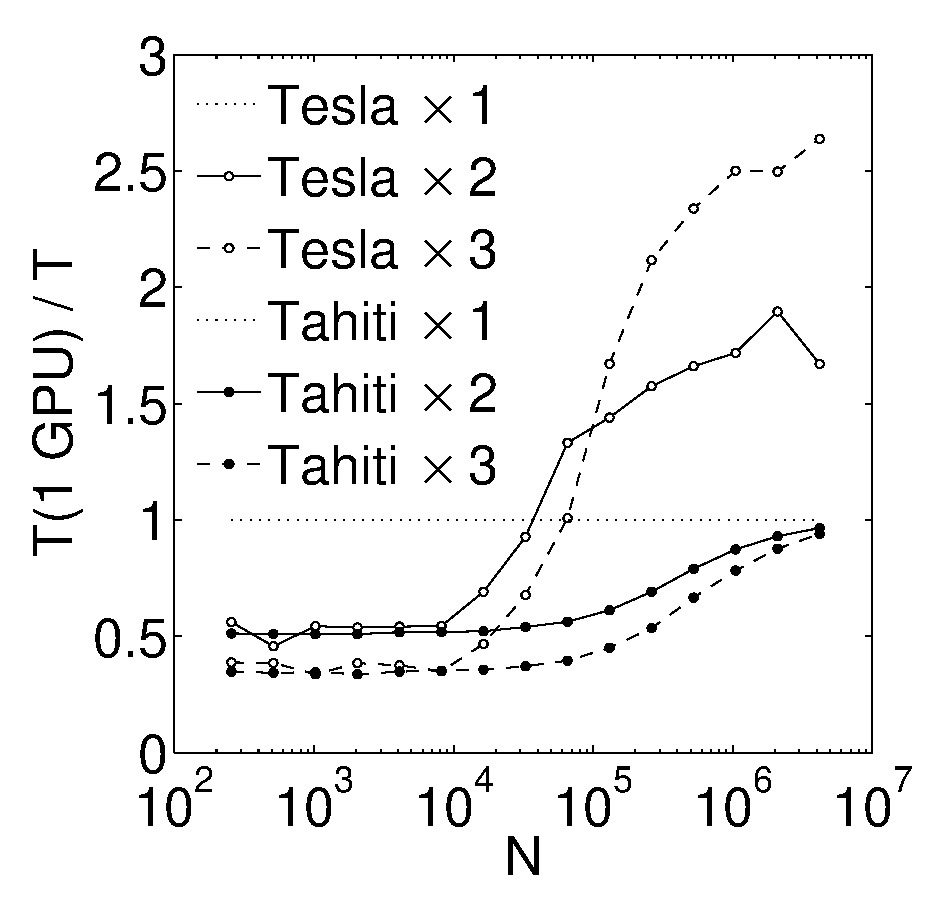
\includegraphics[width=0.45\textwidth]{data/damped_oscillator/scaling}}\quad
        \subfigure[
        Coupled phase oscillator chain
        ]{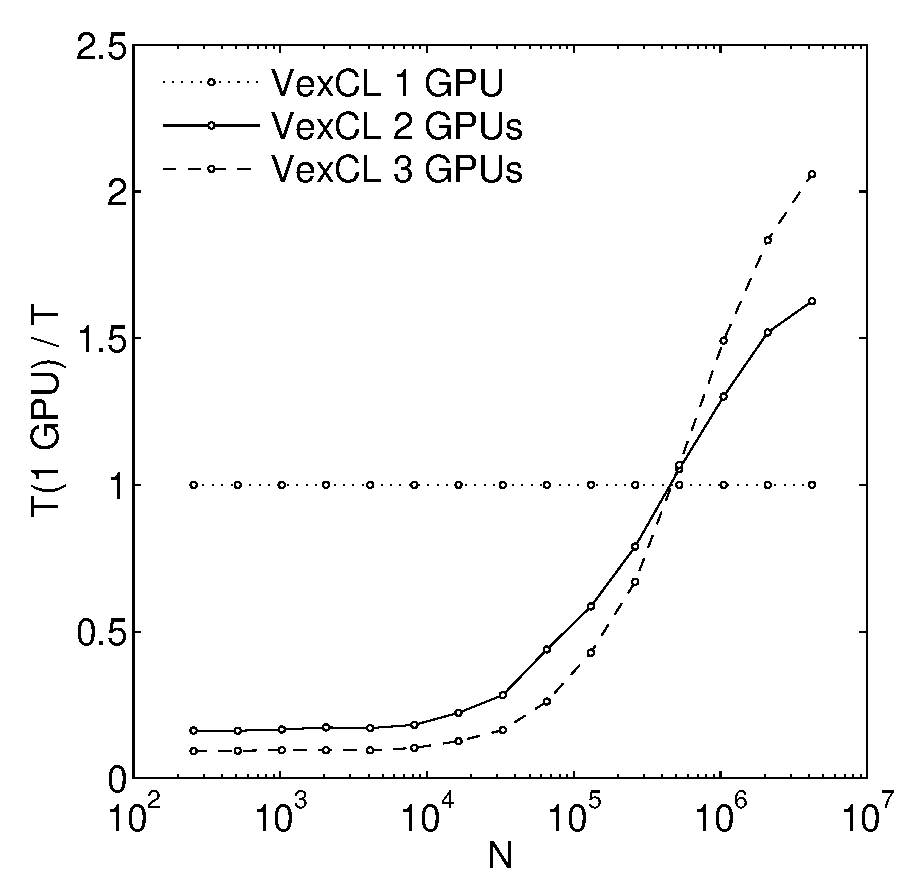
\includegraphics[width=0.45\textwidth]{data/phase_oscillator_chain/scaling}}\\
        \subfigure[
        Disordered Ham lattice
        ]{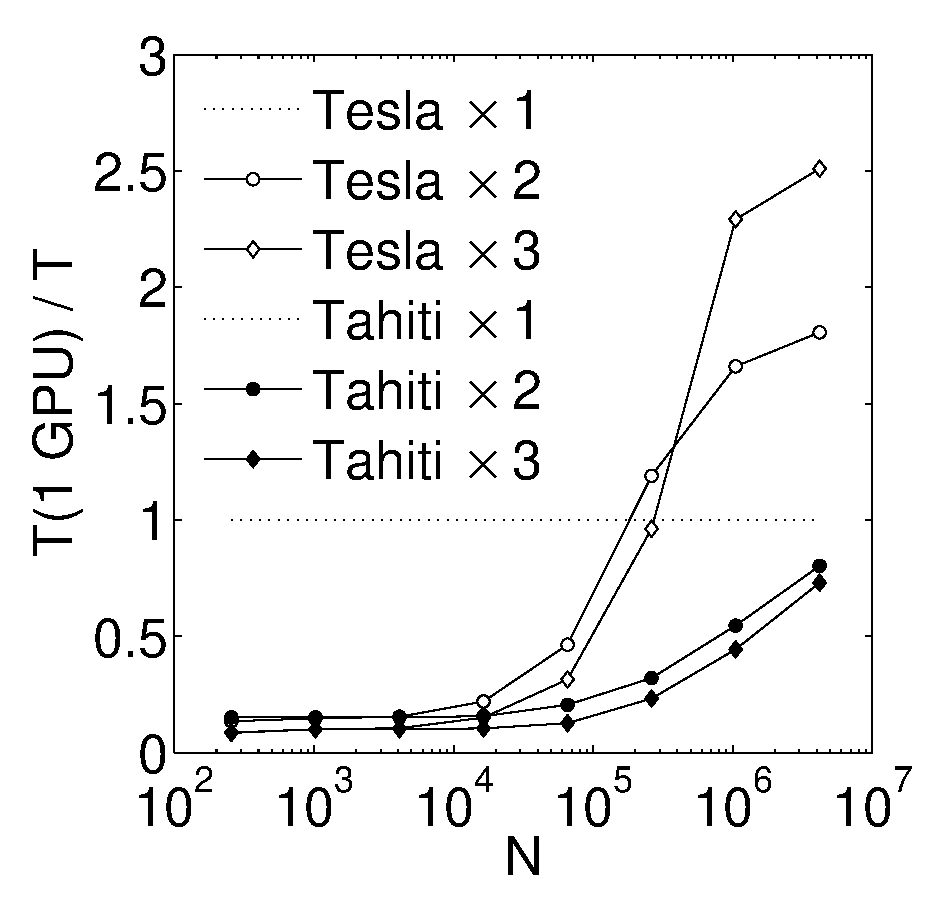
\includegraphics[width=0.45\textwidth]{data/disordered_ham_lattice/scaling}}\quad
        \subfigure[
        Lorenz attractor ensemble
        ]{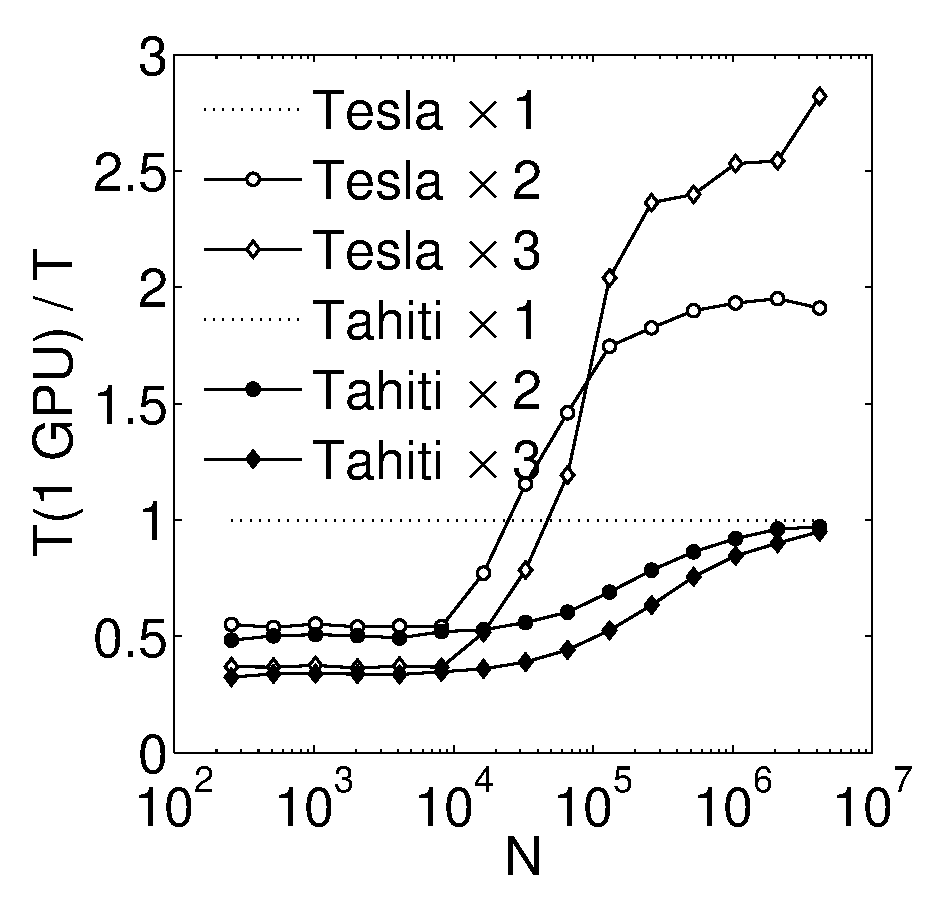
\includegraphics[width=0.45\textwidth]{data/lorenz_ensemble/scaling}}
    \end{center}
    \caption{VexCL scaling with multigpu computation}
    \label{fig:scaling}
\end{figure}









%
% FURTHER OPTIMIZATIOn
%
\section{Further optimizations}

It may be said that performance we got so far is not optimal. Indeed, generic
odeint algorithms use temporary vector variables. For example, fourth-order
Runge-Kutta method used in our examples uses at least four temporary state
variables on each integration step. All of those temporaries are full-blown
vectors that waste global memory reads and writes. 

\begin{figure}[p]
\begin{lstlisting}
double2 system_function(
    double omega, double amp, double offset, double omega_d,
    double dt, double t, double2 s
    )
{
    double eps = offset + amp * cos(omega_d * t);
    double2 dsdt;
    dsdt.x = dt * (eps * s.x + omega * s.y);
    dsdt.y = dt * (eps * s.y - omega * s.x);
    return dsdt;
}
kernel void dumped_oscillator(
    ulong  n, global double *X, global double *Y,
    double omega, double amp, double offset, double omega_d,
    double dt, double t
    )
{
    double2 s, dsdt, k1, k2, k3, k4;
    for(size_t gid = get_global_id(0); gid < n; gid += get_global_size(0)) {
        s.x = X[gid];
        s.y = Y[gid];
        k1 = system_function(omega, amp, offset, omega_d, dt, t, s);
        k2 = system_function(omega, amp, offset, omega_d, dt,
                t + 0.5 * dt, s + 0.5 * k1);
        k3 = system_function(omega, amp, offset, omega_d, dt,
                t + 0.5 * dt, s + 0.5 * k2);
        k4 = system_function(omega, amp, offset, omega_d, dt,
                t + dt, s + k3);
        s += (k1 + 2 * k2 + 2 * k3 + k4) / 6;
        X[gid] = s.x;
        Y[gid] = s.y;
    }
};

\end{lstlisting}
\caption{Hand-coded kernel implementing single iteration of 4th order
Runge-Kutta method.}
\label{code:customkrn}
\end{figure}

It is of course possible to manually create computational kernel corresponding
to the full integration step. \figref{code:customkrn} shows just this
kernel. Unfortunately, by choosing this path we lost generality that odeint
provides.

\begin{figure}[p]
\begin{lstlisting}
typedef vex::generator::symbolic<double> sym_value;
typedef std::array<sym_value,2> sym_state;

struct oscillator {
    double omega, amp, offset, omega_d;
    sym_value &sym_time;
    oscillator(double omega, double amp, double offset,
               double omega_d, sym_value &sym_time)
        : omega(omega), amp(amp), offset(offset), omega_d(omega_d),
          sym_time(sym_time)
    {}
    void operator()(const sym_state &x, sym_state &dxdt, double t) {
        sym_value eps = offset + amp * cos( omega_d * (sym_time + t) );
        dxdt[0] = eps * x[0] + omega * x[1];
        dxdt[1] = eps * x[1] - omega * x[0];
    }
};
\end{lstlisting}
\caption{Symbolic system functor used in automatic kernel generation.}
\label{code:symsysfunc}
\end{figure}

\begin{figure}[p]
\begin{lstlisting}
// Custom kernel body will be recorded here:
std::ostringstream body;
vex::generator::set_recorder(body);

// State types that would become kernel parameters:
sym_state sym_S = {sym_value::VectorParameter, sym_value::VectorParameter};
sym_value sym_time(sym_value::ScalarParameter);

// Symbolic stepper:
odeint::runge_kutta4<sym_state, double, sym_state, double,
        odeint::range_algebra, odeint::default_operations
        > sym_stepper;
oscillator sys(1.0, 0.2, 0.0, 1.2, sym_time);
sym_stepper.do_step(std::ref(sys), sym_S, 0, dt);

// Now that expression sequence is recorded, we build OpenCL kernel:
auto kernel = vex::generator::build_kernel(ctx.queue(),
        "damped_oscillator", body.str(), sym_S[0], sym_S[1], sym_time);

// Actual data (initialization skipped).
vex::vector<double> X(ctx.queue(), n), Y(ctx.queue(), n);

// Integration loop:
for(double t = 0; t < t_max; t += dt) kernel(X, Y, t);
\end{lstlisting}
\caption{Automatic generation of OpenCL kernel corresponding to 4th order
Runge-Kutta method}
\label{code:krnbuilder}
\end{figure}

VexCL library provides kernel generation mechanism that is able to solve this
problem. It allows transparent conversion of generic CPU algorithms
(restrictions applied) to OpenCL kernels. In order to do this conversion one
needs to record sequence of arithmetic expressions made by an algorithm.  The
recording is done with help of \code{vex::generator::symbolic<T>} class. The
class supports arithmetic expression templates and simply outputs to provided
stream any expressions it is being subjected to. This technique is demonstrated
on \figref{code:symsysfunc} and~\ref{code:krnbuilder}. Its advantage is that we
are able to select any stepper from odeint library (or any other generic
algorithm) for the generated kernel. \figref{fig:genkernel} presents
performance comparison of Thrust-based odeint solution with hand-coded and
generated OpenCL kernels. Both hand-coded and generated kernels show very
similar performance and outperform Thrust-based odeint solution by a factor of
5 for large problem sizes. Moreover, generated kernel is slightly faster than
hand-coded kernel. We believe this is due to the fact that VexCL kernel
generator unrolls all operations in the kernel and hard-codes any constants it
encounters in expression sequence.

\begin{figure}[p]
    \begin{center}
        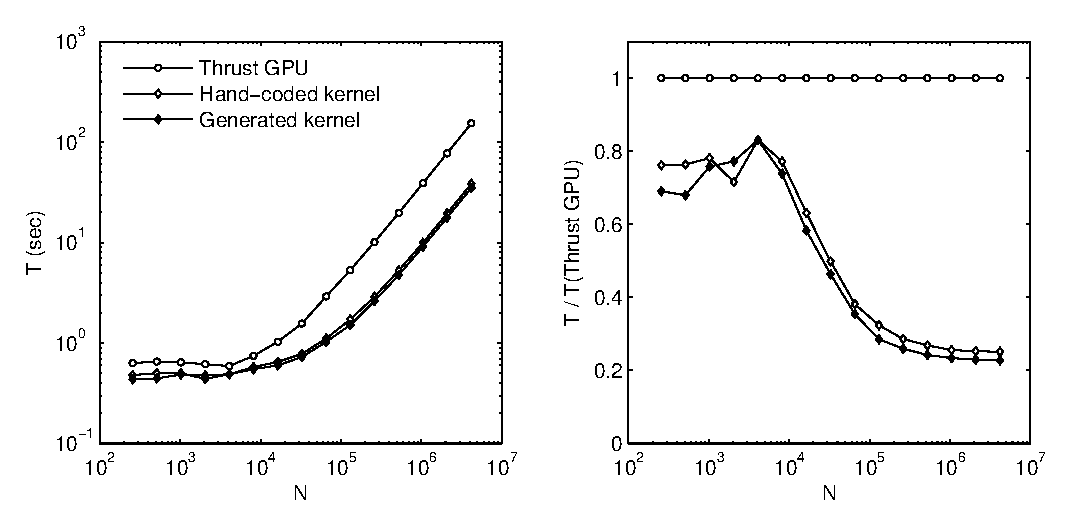
\includegraphics[width=\textwidth]{data/damped_oscillator/genkernel}
    \end{center}
    \caption{Performance of damped oscillator example with hand-coded and
    generated OpenCL kernels compared with Thrust-based odeint solution.}
    \label{fig:genkernel}
\end{figure}








% 
% CONCLUSION
%
\section{Conclusion}

Performance-wise, there is almost no difference between various platforms and
libraries when those are run on the same hardware. As we have shown, various
computational problems may be solved effectively in terms of both human and
machine time with help of modern high level libraries.  There are some
differences in the programming interfaces of the libraries which may be crucial
for ones specific application. 

Thrust is more low level and its interface is very close to C++ STL library.
OpenCL libraries that we looked at provide more convenient interface for a
scientific programmer. VexCL has richer set of elementwise vector operations,
but ViennaCL has extensive set of sparse linear systems solvers (very important
feature which we did not discuss in this paper).

Regarding CUDA vs OpenCL comparison, we believe that OpenCL has two major
advantages with respect to CUDA. First, it has much wider range of supported
hardware which is only going to widen with time, since OpenCL is open standard
supported by major hardware producers. Second advantage of OpenCL is at the
same time its drawback: one has to (or may to) compile his kernels at compile
time. This adds overhead notable for smaller workloads but at the same time it
allows one to transparently build much more effective kernels, as it has been
shown in this paper. 






\section{Acknowledgments}

This work has been partially supported by RFBR grant No 12-07-0007. We also
would like to thank Gradient
JSC\footnote{\href{http://www.gradient-geo.com/en}{http://www.gradient-geo.com/en}}
for the kindly provided AMD hardware.

\bibliographystyle{model1-num-names}
\bibliography{ref}

\end{document}
% vim: set et
